\documentclass{ocbeameruni}


\setdefaultlanguage[babelshorthands=true]{german}


% Nur benötigt für die Beispiel-Listings!
\usepackage{listings}
\usetikzlibrary{arrows}
\lstloadlanguages{[LaTeX]TeX}
\lstset{%
  basicstyle=\small \ttfamily,
  breaklines=true,
}

\newcommand{\R}{\mathbb{R}}


\title{Organic Computing 2}
\subtitle{Lösungsvorschlag Blatt04}
\date{\today}
\author{Lukas Huhn \and Qiang Chang \and Victor Gerling}
\institute{%
  Universität Augsburg\\
  Institut für Informatik\\
  Lehrstuhl für Organic Computing
}


\begin{document}


\maketitle


\begin{frame}{Gliederung}
  \setbeamertemplate{section in toc}[sections numbered]
  \tableofcontents
\end{frame}


\section{Aufgabe 01}

\begin{frame}{1.1.1}
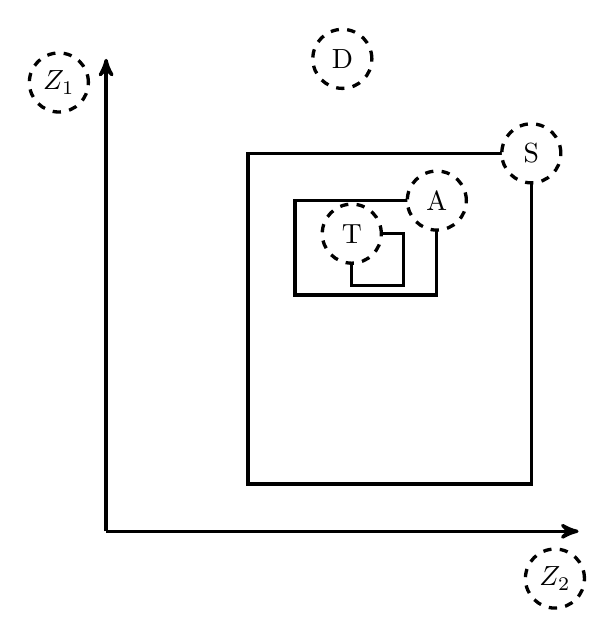
\begin{tikzpicture}[
  >=stealth',
  very thick,
  scale=0.6,
  gap/.style={draw,circle,minimum width=0.75cm,inner sep=0,dashed,fill=white,align=center}
  ]


  \draw[->] (0, 0) -- (0, 10);
  \node [gap] at (-1, 9.5) {$Z_1$};
  \draw[->] (0, 0) -- (10, 0);
  \node [gap] at (9.5, -1) {$Z_2$};


  \node [gap] at (5, 10) {D};
  \draw (3, 1) rectangle (9, 8) node [gap] {S};
  \draw (4, 5) rectangle (7, 7) node [gap] {A};
  \draw (5.2, 5.2) rectangle (6.3, 6.3);
  \node [gap] at (5.2, 6.3) {T};


\end{tikzpicture}
\end{frame}

\begin{frame}{1.1.2}
    \begin{itemize} 
    \item Szenario 1 entspricht Target Space T, weil Fahren mit 180km/h auf der linken Spur die beste Choice ist, damit kann er schnellst nach Hannover ankommen.
    \item Szenario 2 entspricht Transition von Target Space nach Survival Space. Wegen des Knalls von einer der Reifen kann er nicht weiter fahren, sondern ohne 
weitere Schäden auf dem Standsreifen halten.
    \item Szenario 3 entspricht Transition von Survival Space nach Acceptance Space, weil er nach Reifenwechsel weiterfahren kann.
    \end{itemize}
\end{frame}

\begin{frame}{1.1.2}
    \begin{itemize} 
    \item Szenario 4 entspricht Acceptance Space. Er kann jetzt weiterfahren, aber nur auf rechten Spur mit 80km/h.
    \item Szenario 5 entspricht Transition von Acceptance Space nach Target Space. Nach Repair in der Werkstatt kann alles wie Anfangszustand zurückkehren. 
    \item Szenario 6 entspricht Target Space. Jetzt kann er wieder mit 180km/h fahren.
    \end{itemize}
\end{frame}


\begin{frame}{1.1.3}
    \begin{figure}[H]
    \centering
    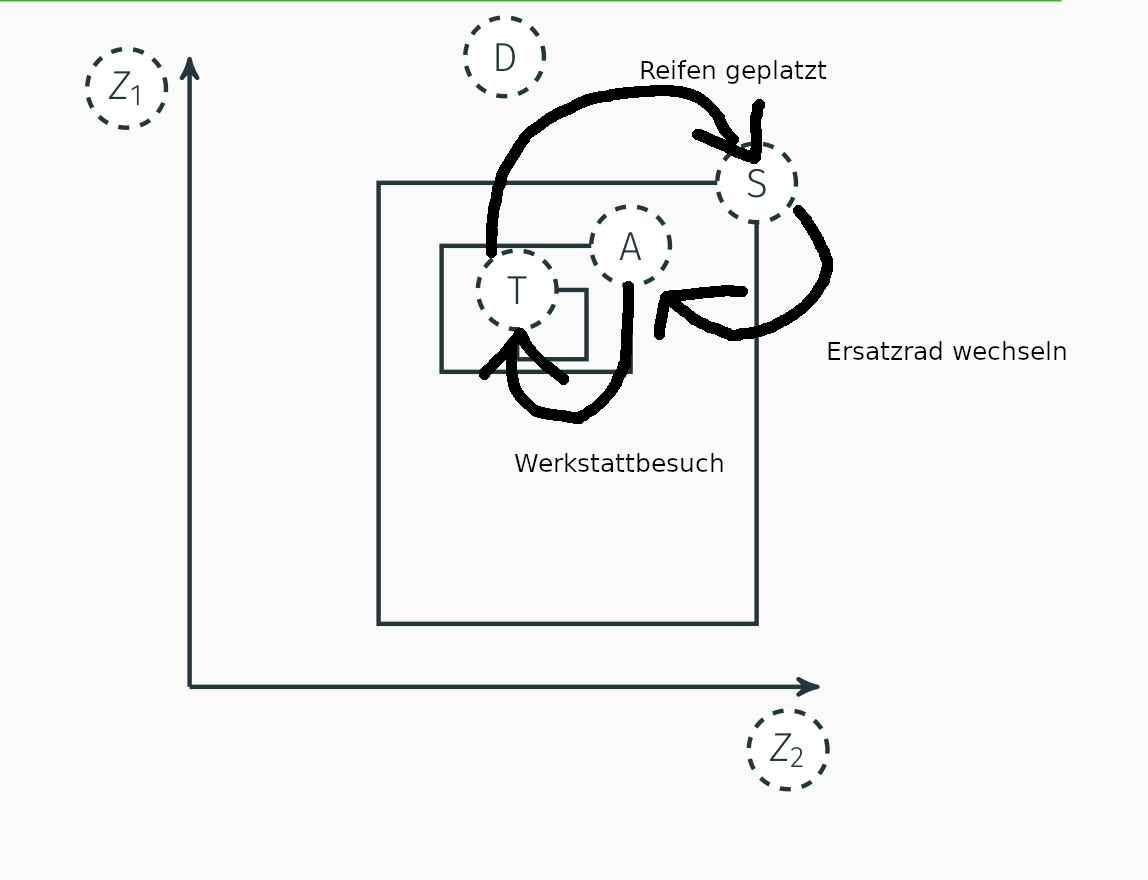
\includegraphics[scale=1.0]{oc_1-1-3.png}
    \end{figure}
\end{frame}

\begin{frame}{1.2.1}
In welchem Zustand befände sich das System, wenn sich das Auto in einem Bereich mit Ge-
schwindigkeitsbegrenzung bewegte (z. B. 120 km/h)?
    \begin{itemize}
    \item Es befände sich im Acceptance space.
    \end{itemize}
\end{frame}

\begin{frame}{1.2.2}
Ist das System robust bezüglich Staus? Bezüglich der Störung aus Aufgabe 1.1? Falls ja, welche
Art der Robustheit liegt vor?
    \begin{itemize}
    \item Bezüglich Staus ist das System nicht robust, bezüglich der Störung aus Aufgabe 1.1 ist es aber weakly robust
    \end{itemize}
\end{frame}

\begin{frame}{1.2.3}
Wie kann man das Szenario so erweitern, dass es auch ein Beispiel für Flexibilität enthält?
    \begin{itemize}
    \item Wegen eines Gewittersturm gibt es jetzt eine Verkehrssteurung bzw. Geschwindigkeitsbegrenzung(80km/h)
    \end{itemize}
\end{frame}

\section{Aufgabe 02}


\section{Aufgabe 03}

\begin{frame}{3.1}
Welche Einheit hat die Utility-Degradation bei dieser Maschine?
    \begin{itemize}
    \item Anzahl gefertigter Stücke
    \end{itemize}
\end{frame}

\begin{frame}{3.2}
    \begin{center}
Zeichnen Sie den zeitlichen Verlauf des Durchsatzes der Maschine und fügen Sie Ihrem Graphen
auch eine Markierung für den Akzeptanzschwellwert hinzu!
    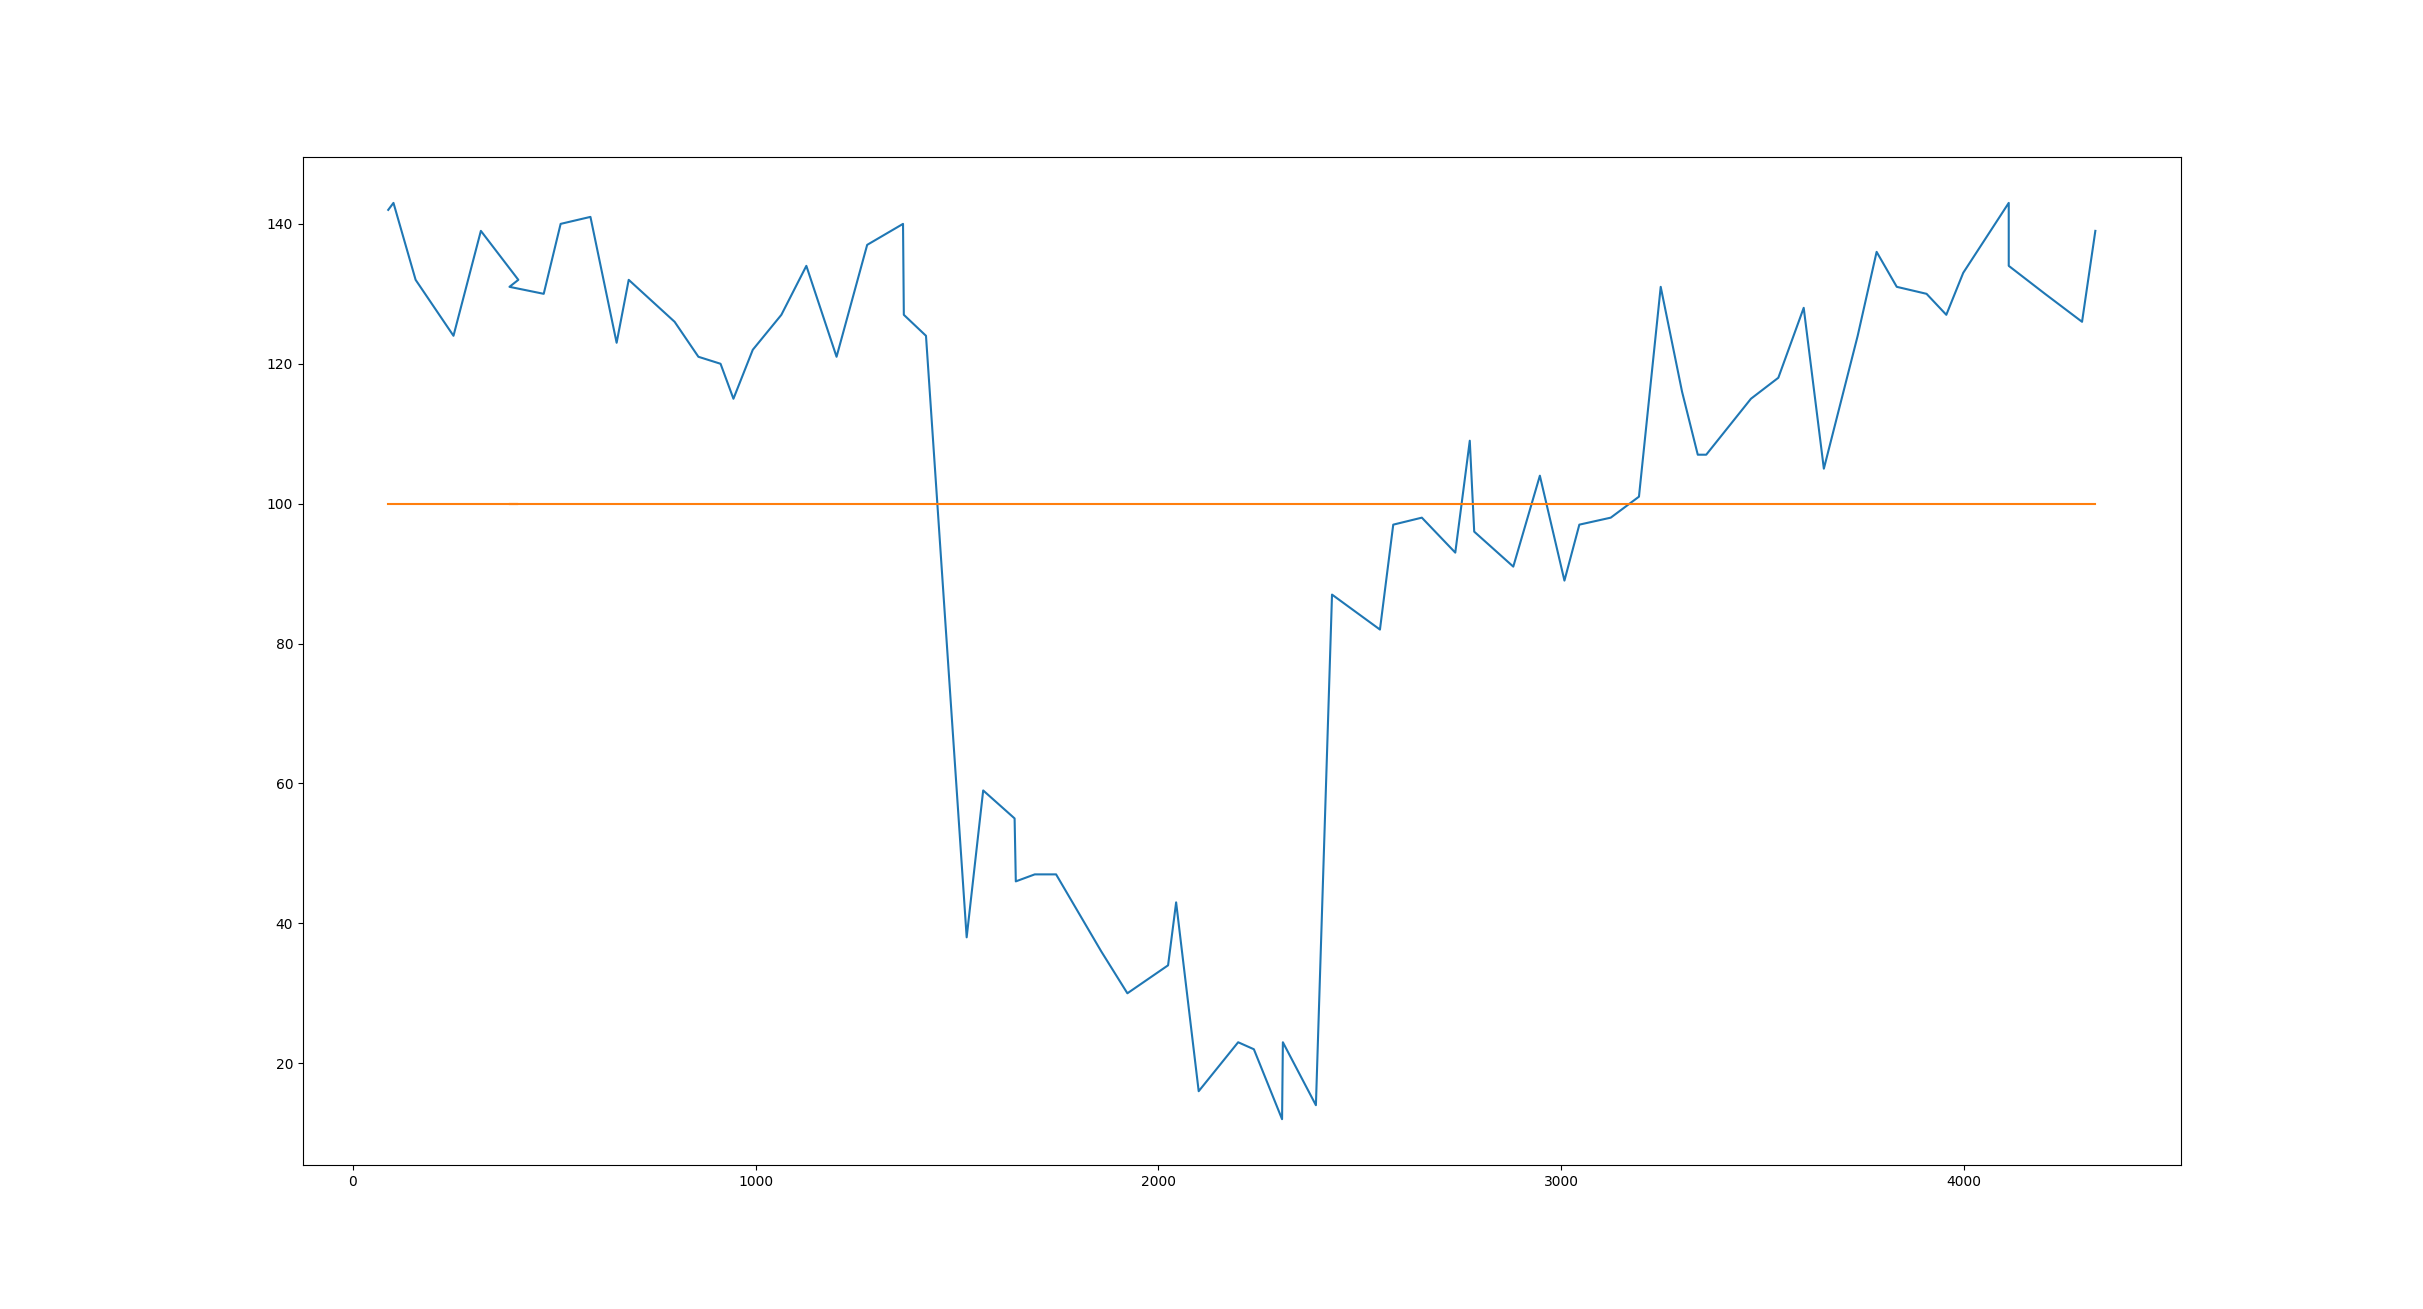
\includegraphics[scale=0.16]{oc_3-2.png}
    \end{center}
\end{frame}

\begin{frame}{3.3}
Berechnen Sie die Utility-Degradation mithilfe der in der Vorlesung vorgestellten Schätzung
mittels eines Dreiecks!
    \begin{itemize}
    \item $D_u = \delta{_u} * t_{rec} / 2 \Rightarrow (100-12) * (3180-2300) / 2 = 38720$
    \end{itemize}
\end{frame}

\begin{frame}{3.4}
Berechnen Sie die Utility-Degradation mithilfe einer näherungsweisen Integration, wie sie in
der Übung vorgestellt wurde!
    \begin{itemize}
    \item $t_{\delta} = 1450, t_{end} = 3180$
    \item $A_1 = (3180-1450)/72 * \sum{_t} U(t) \Rightarrow 1730/72*7290 = 175162.5$
    \item $A_2 = (3180-1450)*100 = 173000$
    \item $D_u = A_2 - A_1 = 173000 - 175162.5 = - 2162.5$
    \end{itemize}
\end{frame}

\begin{frame}{3.5}
Berechnen Sie die Robustheit gegenüber der aufgetretenen Störung (basierend auf 4.)! Benutzen
Sie dazu das in der Übung vorgeschlagene Robustheitsmaß.
    \begin{itemize}
    \item $t_{\delta} = 1450, t_{end} = 3180, t_{accept} = 100, u_{\delta} = 13$
    \item $A_3 = (3180-1450) * (100-13) = 150510$
    \item $A_4 = (3180-1450) * 13 = 22490$
    \item $R_s = (D_u - A_4) / A_3 = (-2162.5 - 22490) / 150510 = -0.163793103$
    \end{itemize}
\end{frame}

\begin{frame}{3.6}
Ist ein Garantiefall aufgetreten, den die Firma geltend machen kann? Warum (nicht)?
    \begin{itemize}
    \item Geg.: Robustheit gegenüber Änderungen in der Luftfeuchtigkeit: 60 %.
    \item Garantie kann geltend gemacht werden, da Robustheitsmaß -0.16 beträgt
    \end{itemize}
\end{frame}

\end{document}
% Local Variables:
% TeX-engine: xetex
% End:
